\chapter{Package Documentation}
\section{Structure}
\label{appendix:package}
The package contains two main directories and three metadata files as depicted in Figure \ref{fig:package-structure}. The first directory is the source code directory, \textit{lib}, containing the domain model, and algorithms for computing MobilityContexts. The second directory is the \textit{test} directory containing unit tests which aid in the process of validating the algorithms. The metadata files are the \textit{CHANGELOG.md} which contains a list of changes made to the package such that an application programmer can keep track of changes to the API. 

\begin{figure}
    \centering
    \begin{verbatim}
        mobility_features
        ├── lib/
        │   ├── mobility_context.dart
        │   ├── mobility_domain.dart
        │   ├── mobility_features.dart
        │   ├── mobility_functions.dart
        │   ├── mobility_intermediate.dart
        │   └── mobility_serializer.dart
        ├── test/
        │   ├── data/
        │   ├── mobility_features_test.dart
        │   └── test_utils.dart
        ├── CHANGELOG.md
        ├── pubspec.yaml
        ├── README.md
    \end{verbatim}
    \caption{The file structure of the Mobility Features Flutter Package}
    \label{fig:package-structure}
\end{figure}

The \textit{pubspec.yaml} contains the package specification including the package name, a description, version, homepage, and a list of dependencies. The dependencies are other packages on which the package depends, as in this case, the Mobility Features Package depends on the \verb|simple_cluster|, \verb|stats| and \verb|path_provider| packages each with a specific version number. The package itself also has such a version number that allows an application developer to import a specific version of the package, for example, if they built their application around a previous release, they may wish to continue depending on that specific release rather than upgrading to the newest version.

\begin{figure}
    \centering
    \begin{minted}{yaml}
        name: mobility_features
        description: Real-time mobility feature calculation
        version: 1.1.5
        homepage: https://github.com/cph-cachet/flutter-plugins/
        
        environment:
          sdk: ">=2.7.0 <3.0.0"
        
        dependencies:
          flutter:
            sdk: flutter
          simple_cluster: ^0.2.0
          stats: ^0.2.0+3
          path_provider: ^1.6.10
        
        dev_dependencies:
          flutter_test:
            sdk: flutter
    \end{minted}
    \caption{The pubspec.yaml file for the Mobility Features Package}
    \label{fig:pubspec}
\end{figure}

Lastly, the README.md file contains instructions for using the package including code snippets and use case examples. 

\section{Publishing}
Distributing a Flutter package is done via the Dart Package Manager, Pub. Pub is essentially a git repository of a package including all versions of that package. When publishing a package the contents of the README file are converted to HTML and are what the user is initially presented with. The README should, therefore, give a brief overview and description of the package, in addition to instructions. Figure \ref{fig:pub-package} shows the latest version of the package hosted at \url{https://pub.dev/packages/mobility_features}.

\begin{figure}
    \centering
    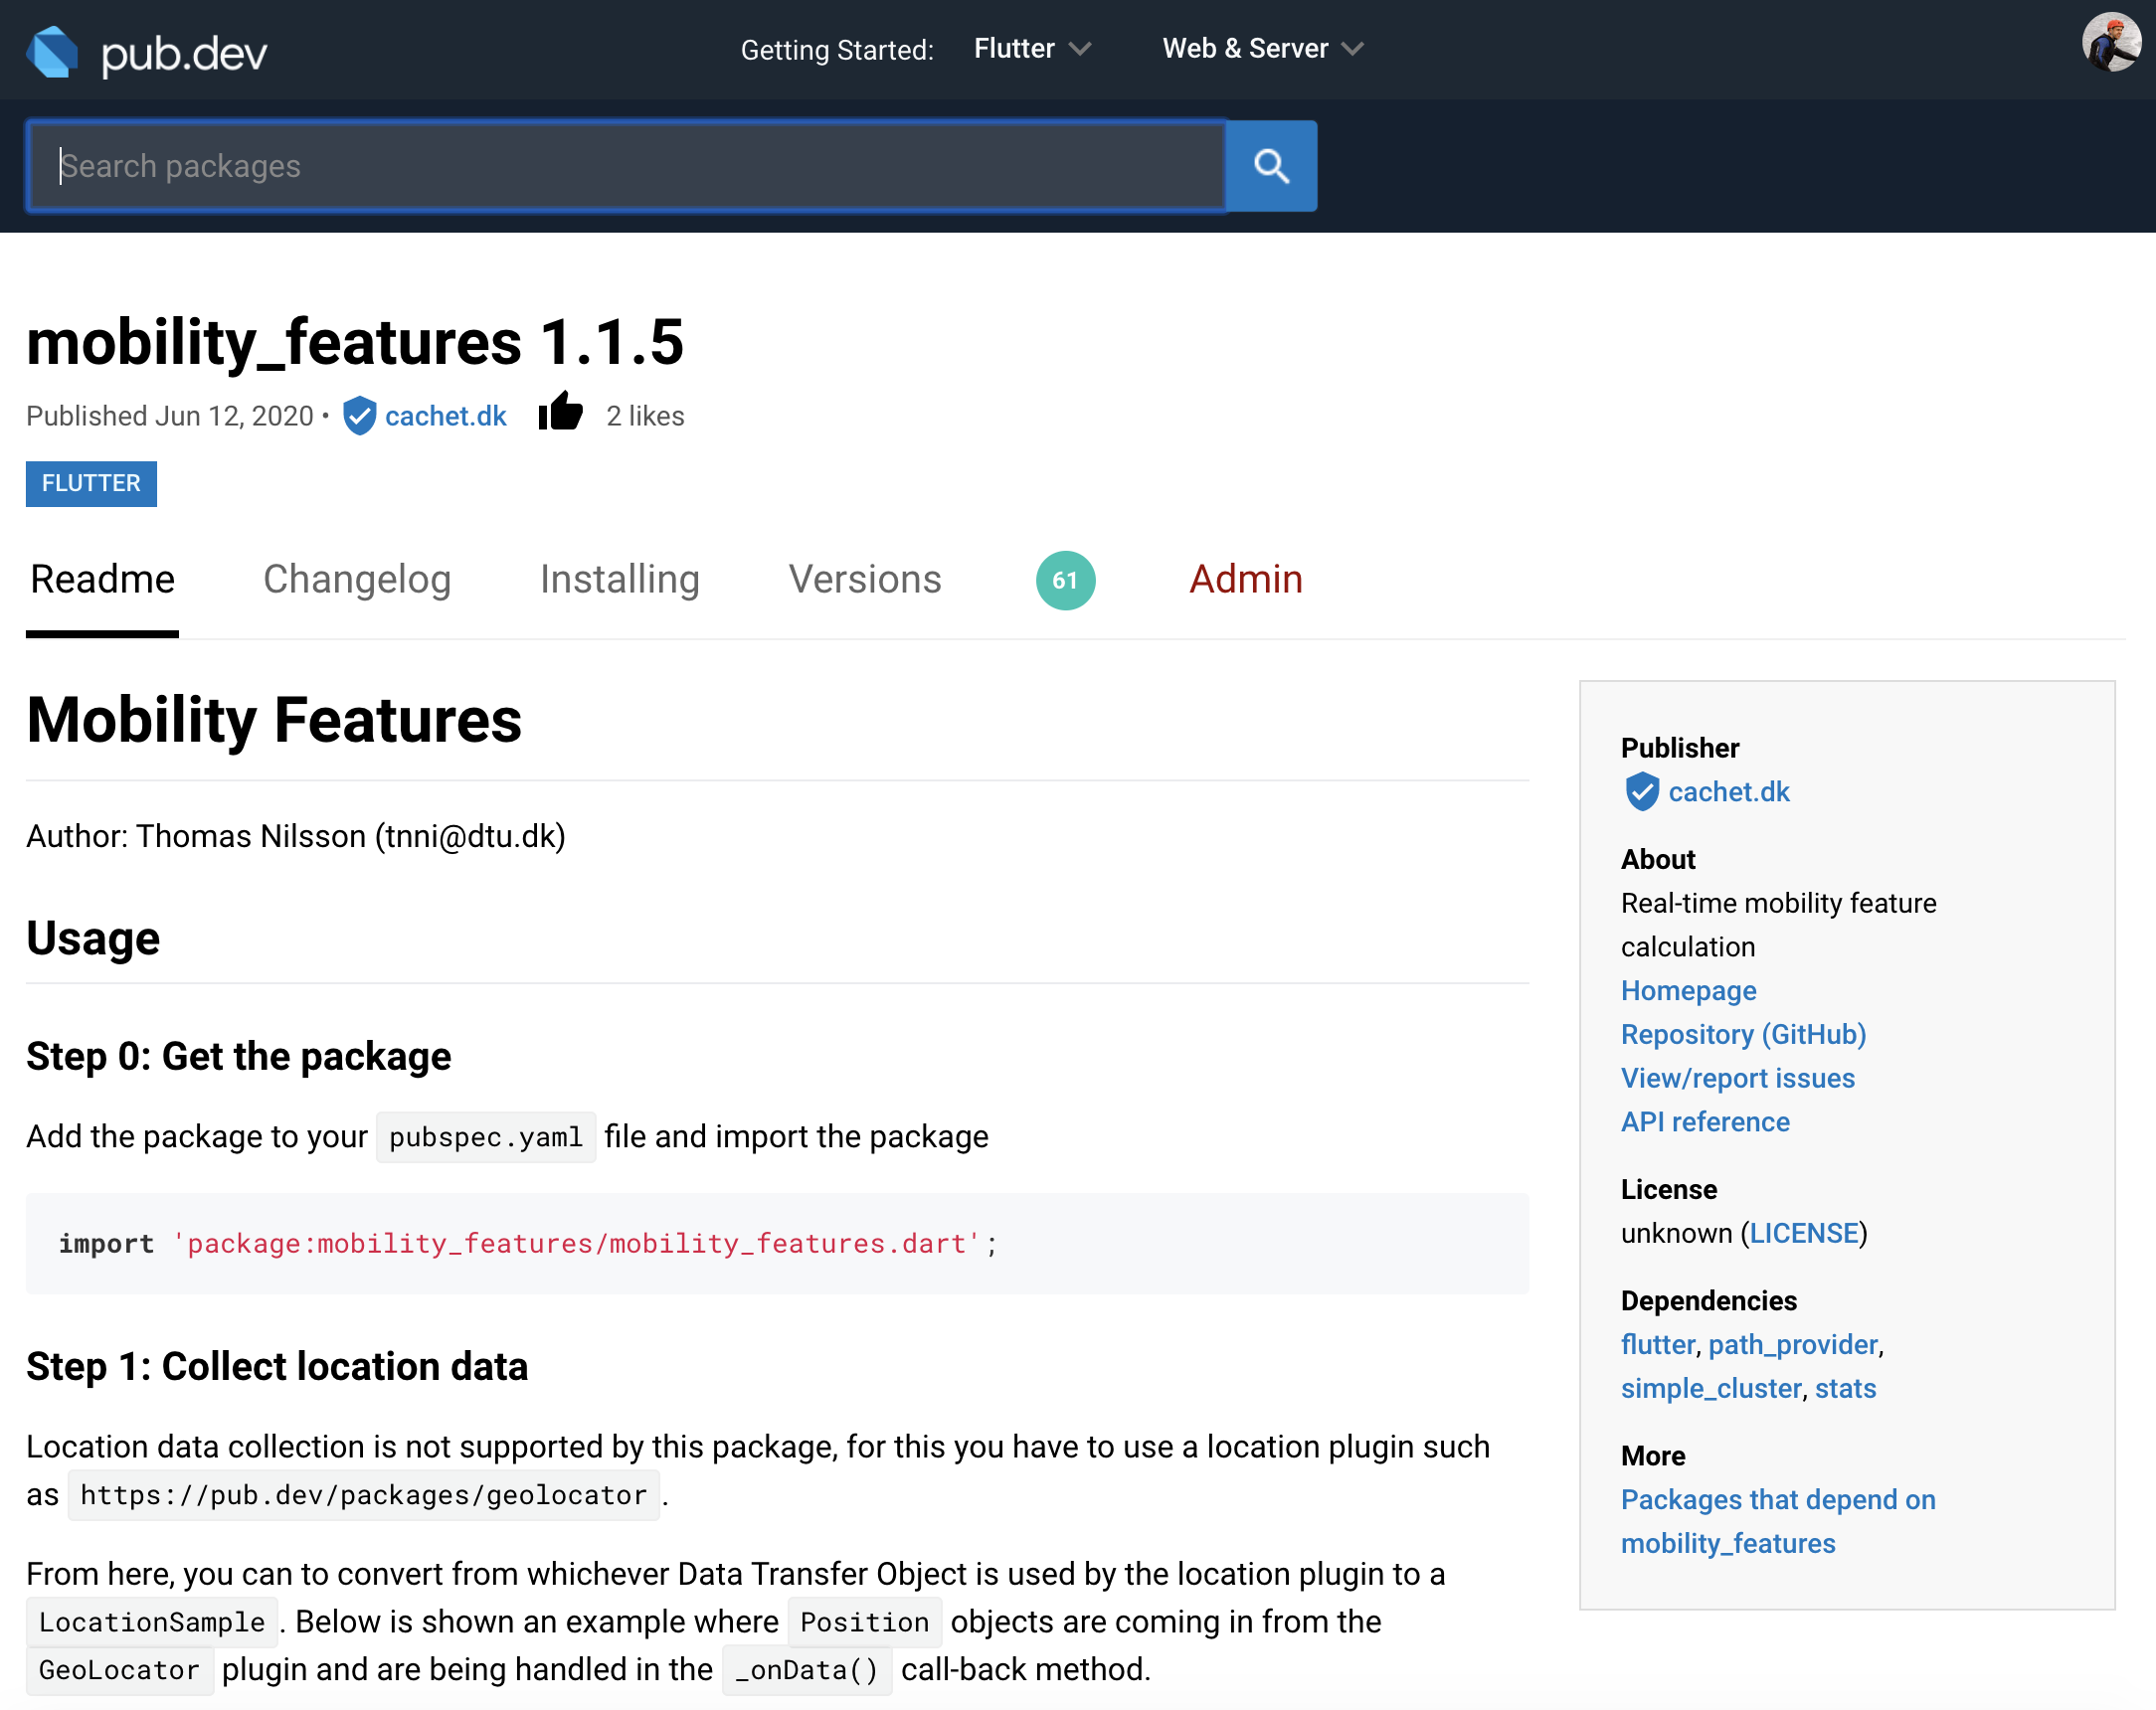
\includegraphics[width=\textwidth]{images/pub.png}
    \caption{The page hosting the Mobility Features Package on www.pub.dev}
    \label{fig:pub-package}
\end{figure}

Publishing automatically generate API documentation by using comments in the code. Normally, comments are made with 2 forward slashes (\textit{//}), but comments made with three forward slashes (\textit{///}) mark the code-block following it with API documentation, i.e. the contents of the comment. 

\begin{figure}
    \centering
    \begin{minted}{dart}
    /// A [LocationSample] holds a 2D [GeoPosition] spatial data point
    /// as well as a [DateTime] value s.t. it may be temporally ordered
    class LocationSample implements _Serializable, _Geospatial {...}
    \end{minted}
    \caption{The API comments for the source code of the Location Sample class}
    \label{fig:api-comments}
\end{figure}

\begin{figure}
    \centering
    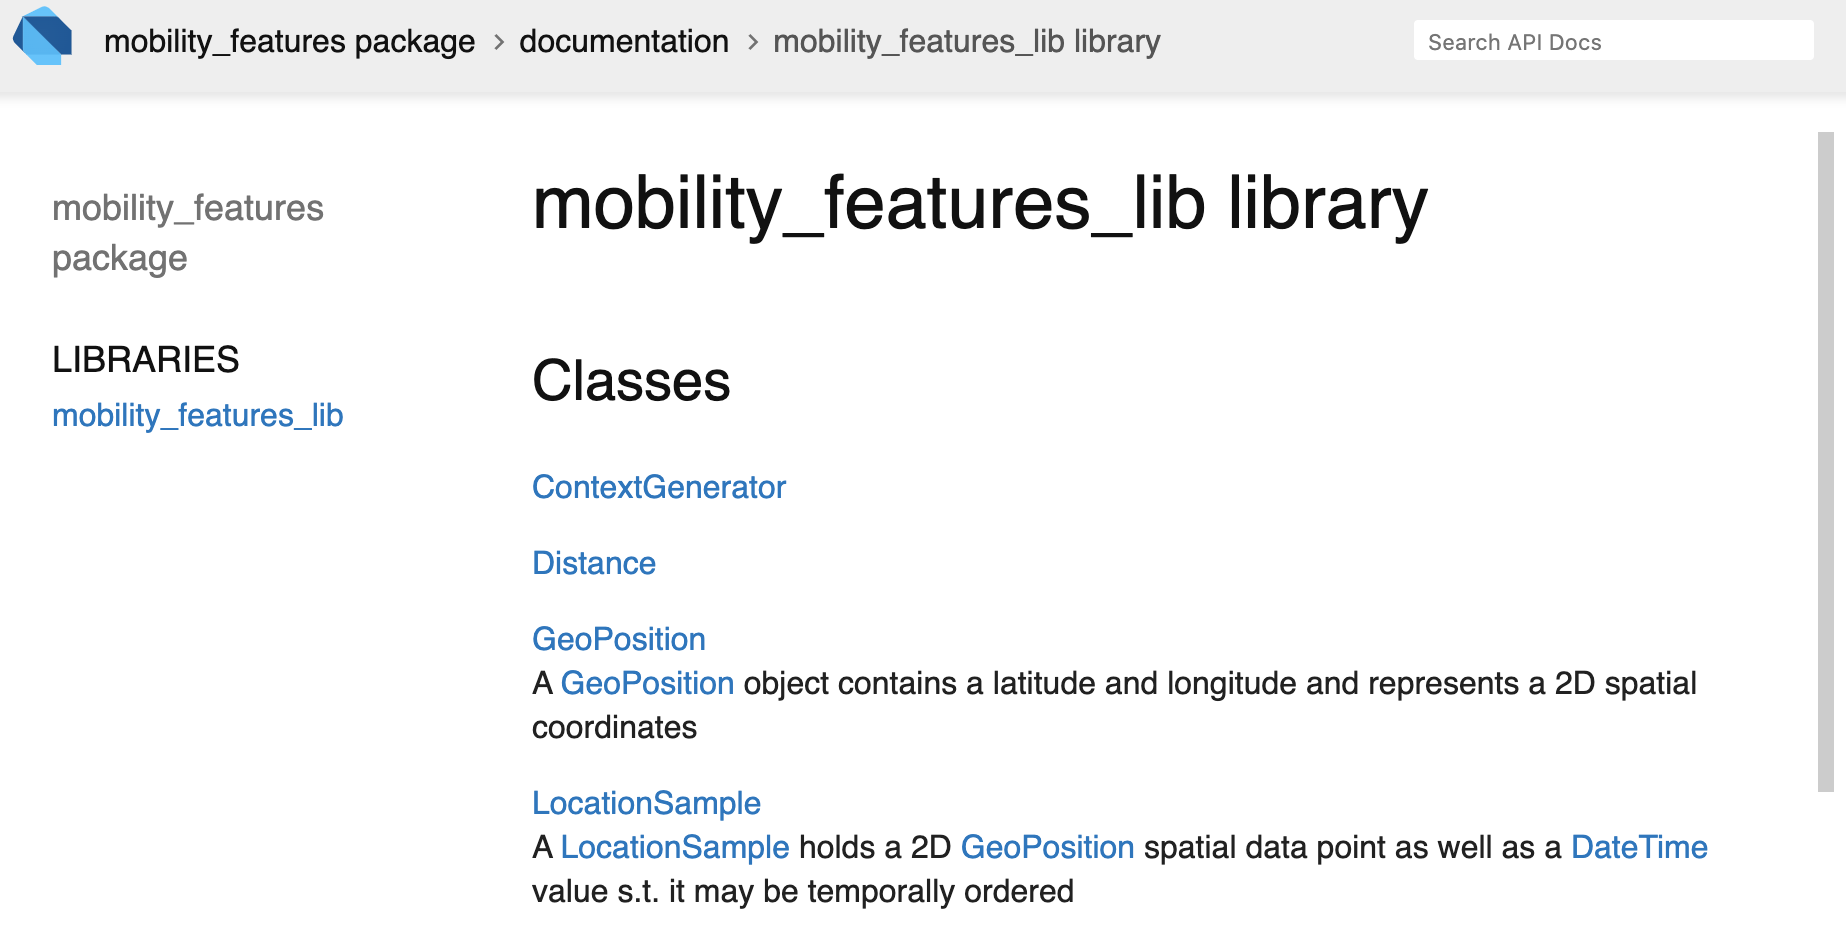
\includegraphics[width=\textwidth]{images/docs.png}
    \caption{The auto generated documentation for the package, hosted on pub.dev, including the code snippet in Figure \ref{fig:api-comments} for the Location Sample class}
    \label{fig:api-docs}
\end{figure}


